\documentclass[12pt]{report}
\usepackage{graphicx}
\usepackage{hyperref}
\usepackage{setspace}
\usepackage{amsmath}
\usepackage{enumitem}
\usepackage{float}
\usepackage{subcaption}
\usepackage{multirow}
\usepackage{adjustbox}
\usepackage{textcomp}
\usepackage{lipsum}
\usepackage{color}
\usepackage{sectsty}
\usepackage[nottoc]{tocbibind}
\usepackage{grffile}
\usepackage{fancyhdr}
\usepackage{acro}
\usepackage[a4paper,includeheadfoot,margin=2.5cm]{geometry}
\pagestyle{fancy}
\usepackage{titlesec}
\usepackage{graphicx}
\usepackage{xcolor}
\usepackage{dirtree}
\usepackage{amssymb}
\usepackage{tikz}
\usepackage{pgfplots}
\graphicspath{{images/}}
\renewcommand{\headrulewidth}{0pt}
\usepackage{listings}
\usepackage{algorithm}
\usepackage[noend]{algpseudocode}
\usepackage{tabu}
\usepackage[scientific-notation=true]{siunitx}
\usepackage{hyperref}
\usepackage{microtype}
\usepackage{tikzsymbols}
\usepackage{makecell}
\usetikzlibrary{matrix,chains,positioning,decorations,arrows}
\emergencystretch=1em
\newcolumntype{M}[1]{>{\centering\arraybackslash}m{#1}}
\newlist{steps}{enumerate}{1}
\setlist[steps, 1]{label = Step \arabic*:}
\newcommand\myicon[1]{{\color{#1}\rule{2ex}{2ex}}}
\newcommand{\myfolder}[2]{\myicon{#1}\ {#2}}

%New colors defined below
\definecolor{codegreen}{rgb}{0,0.6,0}
\definecolor{codegray}{rgb}{0.5,0.5,0.5}
\definecolor{codeyellow}{rgb}{0.85, 0.65, 0.13}
\definecolor{backcolour}{rgb}{0.95,0.95,0.92}

%Code listing style named "mystyle"
\lstdefinestyle{mystyle}{
	backgroundcolor=\color{backcolour}, commentstyle=\color{codegreen},
	keywordstyle=\color{blue},
	numberstyle=\tiny\color{codegray},
	stringstyle=\color{codeyellow},
	basicstyle=\footnotesize,
	breakatwhitespace=false,         
	breaklines=true,                 
	captionpos=b,                    
	keepspaces=true,                 
	numbers=left,                    
	numbersep=5pt,                  
	showspaces=false,                
	showstringspaces=false,
	showtabs=false,                  
	tabsize=2
}

%"mystyle" code listing set
\lstset{style=mystyle}

\usepackage[toc,page]{appendix}
%\usepackage[sorting=none]{biblatex}
%\addbibresource{ref.bib}

\DeclareAcronym{ML}{
  short = ML,
  long  = Machine Learning,
  class = abbrev
}
\DeclareAcronym{SL}{
  short = SL,
  long  = Supervised Learning,
  class = abbrev
}
\DeclareAcronym{UL}{
  short = UL,
  long  =Unsupervised Learning,
  class = abbrev
}
\DeclareAcronym{DL}{
  short = DL,
  long  = Deep Learning,
  class = abbrev
}
\DeclareAcronym{CNN}{
  short = CNN,
  long  = Convolutional Neural Network,
  class = abbrev
}
\DeclareAcronym{RNN}{
  short = RNN,
  long  = Recurrent Neural Network,
  class = abbrev
}
\DeclareAcronym{THS}{
  short = THS,
  long  = Twitter Health Surveillance,
  class = abbrev
}
\DeclareAcronym{HDFS}{
  short = HDFS,
  long  = Hadoop Distributed File System,
  class = abbrev
}
\DeclareAcronym{NIH}{
  short = NIH,
  long  = National Institutes of Health,
  class = abbrev
}
\DeclareAcronym{AI}{
  short = AI,
  long  = Artificial Intelligence,
  class = abbrev
}
\DeclareAcronym{US}{
  short = US,
  long  = United States,
  class = abbrev
}
\DeclareAcronym{NSF}{
	short = NSF,
	long  = National Science Foundation,
	class = abbrev
}
\DeclareAcronym{CSV}{
  short = CSV,
  long  = Comma Separated Values,
  class = abbrev
}
\DeclareAcronym{API}{
  short = API,
  long  = Application Program Interface,
  class = abbrev
}
\DeclareAcronym{GPU}{
  short = GPU,
  long  = Graphic Processing Unit,
  class = abbrev
}
\DeclareAcronym{NLP}{
  short = NLP,
  long  = Natural Language Processing,
  class = abbrev
}
\DeclareAcronym{MLP}{
	short = MLP,
	long = Multilayer Perceptron,
	class = abbrev
}
\DeclareAcronym{UPRM}{
	short = UPRM,
	long  = University of Puerto Rico Mayag\"uez Campus,
	class = abbrev
}

\pgfplotsset{compat=1.15}
\setlength{\headheight}{15pt}
\begin{document}
\newtheorem{definition}{Example}

\pagenumbering{roman}%

\begin{titlepage}
    \centering 
    {\LARGE \textbf {Find Similar Tweets Within Health Related Topics}\par}
    \vspace{1cm}
    {By\par}
    {Danny Gilberto Villanueva Vega\par}    
    {A thesis submitted in partial fulfillment of the requirements for the degree \par}
    \vspace{.1cm}
    {of\par}
    \vspace{.1cm}
    {MASTER OF SCIENCE\par}
    {in\par}
    {COMPUTER ENGINEERING\par}
    {UNIVERSITY OF PUERTO RICO
    \\MAYAG\"UEZ}{  CAMPUS\par}
    {2019}
    \vspace{.1cm}
    \begin{flushleft}
      Approved by:\\
      \vspace{1cm}
    \end{flushleft}
    \begin{tabular}{l c c c c c r}
     
      \rule{2.5in}{.1pt} & & & &  &\rule{2in}{.1pt}\\
      Manuel Rodr\'iguez Mart\'inez, Ph.D. & & & &  &Date\\
      President, Graduate Committee\\
      \vspace{.3cm}\\
      \rule{2.5in}{.1pt}& & & &  &\rule{2in}{.1pt}\\
      Wilson Rivera Gallego, Ph.D. & & & &  &Date\\
      Member, Graduate Committee\\
      \vspace{.3cm}\\
      \rule{2.5in}{.1pt} & & & &  &\rule{2in}{.1pt}\\
      Bienvenido J Velez Rivera, Ph.D. & & & &  &Date\\
      Member, Graduate Committee\\
      \vspace{.45cm}\\
      \rule{2.5in}{.1pt} & & & &  &\rule{2in}{.1pt}\\
      Graduate School & & & &  &Date\\
      Graduate School Representative\\
      \vspace{.45cm}\\
      \rule{2.5in}{.1pt} & & & &  &\rule{2in}{.1pt}\\
      Chairperson, Ph.D. & & & &  &Date\\
      Department Chairperson \\
    \end{tabular}
\end{titlepage}

\setcounter{page}{2}

\addcontentsline{toc}{chapter}{Abstract}
\begin{center}
\doublespacing
Abstract of Thesis Presented to the Graduate School\\
of the University of Puerto Rico in Partial Fulfillment of the\\
Requirements for the Degree of Master of Science in Computer Engineering\\
\vspace{.1cm}
\large\textbf {Find Similar Tweets Within Health Related Topics}
\end{center}
\doublespacing
here abstract of thesis.\\
Here abstract of thesis.\\	
Here abstract of thesis.\\
\par
\clearpage

\addcontentsline{toc}{chapter}{Abstract (Spanish)}
\begin{center}
Resumen de tesis presentada a la Escuela Graduada\\
de la Universidad de Puerto Rico como requisito parcial de los\\
requerimientos para el grado de Maestr\'ia en Ciencias en Ingenier\'ia de Computadoras\\

\vspace{.1cm}
\large\textbf {Encontrar tweets similares en temas relacionados con la salud}
\end{center}
\doublespacing
Aqu\'i resumen de tesis.\\
Aqu\'i resumen de tesis.\\
Aqu\'i resumen de tesis.\\
\par
\clearpage

\vspace*{\fill}
\begin{table}[H]
	\centering
	\begin{adjustbox}{max width=\textwidth }
		\begin{tabular}{c}
			Copyright \textcopyright\hspace{0.15cm}2019 \\
			\textit{by}\\
			\textit{Danny Gilberto Villanueva Vega}\\
		\end{tabular}
	\end{adjustbox} 
\end{table}
\vfill
\clearpage

\vspace*{\fill}
\begin{center}
	\textit{DEDICATION}\\
	\vspace{2cm}
	\textit{To my Mom, Carin Vega P\'erez. To my sister, Emyli S Rodriguez Vega.}
\end{center}
\vfill
\clearpage

\vspace*{\fill}
\addcontentsline{toc}{chapter}{Acknowledgment}

\begin{center}
	\Large \textbf{Acknowledgments}
\end{center}
to thank family\\
\\
to thank advisor\\

This research is supported by the \ac{US} National Library of Medicine of the \ac{NIH} under award number R15LM012275. The content is solely the responsibility of the authors and does not necessarily represent the official views of the \ac{NIH}. Some results presented in this thesis were obtained using the Chameleon Cloud supported by the \ac{NSF}.
\vfill
\doublespacing

\tableofcontents{}

\newpage
\printacronyms[include-classes=abbrev,name=List of Abbreviations]
\newpage
\listoffigures{}
\newpage
\listoftables{}

\newpage
\titlespacing{\chapter}{0pt}{*1}{*1}

\fancyhf{}
\fancyhead[R]{\thepage} 
\renewcommand{\figurename}{Fig}
\pagenumbering{arabic}
\onehalfspacing
\chapter{Introduction}\label{Chapter 1}
\doublespacing

\section{Motivation}
	Social networks have become a very important means to share ideas, discuss news, and opinions on many topics.  They also provide real-time information on sales, marketing, politics, natural disasters, and crisis situations, among others. These networks include Facebook, Twitter, WhatsApp, and Instagram, to name a few. 
	
	In this work, we shall focus our efforts on the Twitter social network. This network provides a mechanism for people to express their views using short messages (i.e., 280 characters)
	called {\em tweets}. 
	Users of this network can find each other messages without the need of becoming ``friends'', as happens in other networks. The analysis of these tweets can enable us to understand the current situation regarding certain topics, for example, discussions related to medical topics (e.g., ``flu'').
	Using the tweets, users can monitor and find patterns that give information about some type of disease being discussed in the social network. In addition, it is possible to detect the position,
	``mood'', or sentiment of the people around some topic.
	
	For the analysis of all this available information it is necessary to group or categorize the text along similarities in structure and  or meaning. However, this is a challenging task, due to the complexity/ambiguity introduced by  spelling errors or the use of informal language (``slang'').  In the case of tweets, the small size of the message often makes it difficult to analyze without the context provided by previous messages or user interactions. Making use of the data stored in the  \ac{THS} System at /ac{UPRM} , as one of our sources, it is possible to process all the information more easily and quickly, and use it to analyze and process the data using  \ac{ML} algorithms.
	
	The view of the world has changed with the presence of \ac{AI} in our lives, we live in a new world surrounding by \ac{ML} (e.g. Amazon Alexa, writing correctors). Companies like Google, Amazon, Netflix and others are using \ac{AI} algorithms to obtain value and insight of large amount of data that in otherwise will been impossible to analyze. The value of the information has been ever the key for the growth of companies; therefore, text analysis is a rough task aim to extract value information to use in business decisions, however this is challenging job due to complexity of \ac{NLP} a field of \ac{ML}  focuses on analyzing the human language.
	
	The detection of similarity in texts in their meaning of semantics content is a topic present in many researches because the need to obtain valuable and reliable information from the amount of available data over internet like, communication services (e.g. “Twitter”), feedback user, system log files, customer reviews to mention a few; and the data present in the same company about employees, clients and others. 
	
	In this project, we investigate and implement text similarity algorithms in such a way that we can: 1) know if they are related or not with a disease, 2) group similar tweets to those that we have already captured, analyzed or stored and, 3) find similarity index between tweets using different learning algorithms. We based our work on, semantic similarity approaches and text similarity measures using \ac{DL} algorithms to deliver reliable information to the end user about health-related topics.
	
	
\section{Objectives}
\begin{itemize}[nolistsep]
	\item \textbf{Collect and filter the data file: } We select necessary tweets and filter all them which are related to health disease thereby, we use a clean data as input to train the algorithms to be implemented. Tweets were collected using \ac{THS} System at \ac{UPRM}. In this way, it is convenient to describe the steps through the process of data selection until deliver of final cleaned up inputs. Part of inputs is labeled data by hand; thus, it is necessary a group of people to classify a measure of similarity between tweets that will be used in training sample.
	\item \textbf{Investigate and implements \ac{DL} algorithms for text similarity measures} It is necessary investigate the state-of-the-art methods and techniques related to text analysis, and then build a robust architecture using \ac{DL} algorithms like, \ac{CNN} and \ac{RNN} on \ac{NLP} approaches,  focusing in text similarity measures. The output of our trained models will be one of two of next options a) there is an acceptable similarity measure between the pair of tweets and, b) no exist enough similarity between the pair of tweets.
	\item \textbf{Test algorithms in a Big Data environment: } The algorithms will be tested to measure the performance and accuracy of results in \ac{THS} cluster located in the Electrical and Computer Department at \ac{UPRM}. Because \ac{DL} algorithms consume a lot of resources, we also use virtual environments as Chameleon Cloud Platforms to test algorithms with better Graphic Processing Unit (GPU) resources than physical machines.
\end{itemize}

\section{Contributions}
\begin{itemize}[nolistsep]
	\item \textbf{Use social networks to get valuable information about health topics:} All data present on internet through social networks, entertainment apps and others, can be used in health-related research. In our case twitter is a source of amount of data of different topics that can be transform in important information relevant for medical issues. Here is showed how we can use data of medical conditions to build models able to compute the similarity in tweets therefore these could be used in future to support on medical applications. 
	\item \textbf{Present \ac{DL} models for text similarity analysis:} \ac{DL} models are very powerful for analysis of data like images, sound, and text. In this project, we try to use these excellent tools of \ac{ML} to figure out a better text similarity model.
	\item \textbf{Employ Supervised Learning in text similarity tasks:} Many studies about sentence representation (“encoding models”) is based in Unsupervised Learning because there is not enough labeled data about a specific topic to train a model like in our case, with data diseases related. We show the trained models with labeled data in sentence similarity has enough performance to be widely adopted in others \ac{NLP} tasks.
	\item \textbf{Use different measure of similarity:} In this project we used three methods to calculate similarity text. Most known is cosine similarity, also Frobenius Distance and our own distance measure called Triangular UL Distance based in part of linear algebra, in a special kind of square matrix called triangular matrix.
	\item \textbf{Describe the evaluation of similarity models: } We built models with \ac{CNN}, \ac{RNN} and merged approaches to get better results. They were tested with different setting to find the best model possible, we used the next metrics F1-Score, Precision and Recall.
\end{itemize}

\section{Outline}
The outline of this thesis is as follows. Chapter 2 contains the literature review about concept of \ac{ML} and \ac{DL} to contextualize the presented solution. In this chapter also in describe topics of \ac{NLP} and text similarity methods. The problem description and the methodology followed to get the similarity models is described in Chapter 3. In Chapter 4, explains the \ac{ML} architecture and describe the different \ac{DL} models built using \ac{CNN} and \ac{RNN} approaches. Chapter 5 shows the result of performance and accuracy of all models described on above chapter. Finally, Chapter 6 shows the conclusions and future work to follow.

\onehalfspacing

\chapter{Literature Review} \label{chapter 2}
\section{Introduction}
Advance of technology has been many changes in the world and our life is now surrounding for \ac{ML} algorithms hence, companies of all sizes are following the large business' success using \ac{AI} to draw insight that can be used to take better decisions.

The field of \ac{AI} seeks to understand how humans think (``intelligence'') and how build intelligent entities. Then what we use \ac{AI} today for? Because the wide field, there is no a simple answer, but we can mention a few applications next, robotic vehicles, speech recognition, autonomous planning and scheduling, game playing, spam fighting, logistics planning, robotics, machine translation, to mention a few applications that exist today, combining efforts of science, engineering and mathematics \cite{Russell2010}.This applications need process a lot of data, hence it is necessary automate the process of analysis, here \ac{ML} appears like a subfield of \ac{AI} that automate the process of learning extracting patterns from the raw data to get insight \cite{Kelleher2015}.

Artificial Neural Networks are simply a collection of connected units that represent abstractly the human brain (“neurons”) to aim achieve learning a specific task \cite{Russell2010}. In this project we are working on similarity tasks. Today exist many applications of similarity like handwritten digits recognition, similarity images detection from text or an image in the web searchers (e.g. Google, Bing). Generic Neural Network techniques can be successfully applied for these problems, but to achieve better result and scale to large applications we need used techniques specialized on certain domains, for example in case of \ac{NLP} (``text analysis'') we need methods to process sequential data, like {RNN}, that is a{DL} technique part of {ML} field. \cite{Goodfellow2016}

\section{Machine Learning}

\ac{ML} also knows as automated learning is associated with the concept of “to learn”, this learning is composed of an input data that represent experience, using a learning algorithm is achieved an output with some expertise \cite{Shai2014}. This learning is focus in gain knowledge, understanding, experience and skills \cite{Nilsson1998} in such a manner its performance improves significantly.

Today we look that \ac{ML} is in many practical applications that we use in frequently in our daily life like: movie recommendation, text translation, speech recognition \cite{Goodfellow2016}, robotic vehicles, autonomous planning and scheduling, diagnosing diseases \cite{Russell2010}. In essence, we are speaking about \ac{ML} when an artificial intelligence system has the ability or capability to get knowledge or find patterns from raw data \cite{Goodfellow2016}. \ac{ML} study data to detect patterns to be able to categorize, predict, identify unknown pattern and detect anomalies or unknown patterns, because Big Data we now have the advantage to process an amount of data, and using {ML} algorithms we can identify new opportunities to solve complex problems like self-driving cars, fraud detection, virtual assistants, resource optimization and more applications \cite{Nevala2017}.

\ac{ML} is a very wide field, for this reason it has branched into several sub-fields related to distinct tasks \cite{Shai2014} and approaches to solve problems. For the study and application of these algorithm exist many ways to classify the learning paradigms, the best known is supervised learning and unsupervised learning, this distinction is by what kind of experience they are allowed to have during the learning process \cite{Goodfellow2016}, others kinds of {ML} are semi-supervised learning and reinforcement learning.


\subsection{Supervised Learning}

Supervised Learning is based in an set of input-output pairs, these models learn automatically of the relationship between input features and target features, through a function that maps from the input data to output feature \cite{Russell2010} \cite{ Kelleher2015}. This kind of learning is only possible if we know the target of the output data \cite{Nilsson1998}, and if we have the enough input labeled data to train the {ML} algorithm.

More abstractly, Supervised Learning describe a scenery where the training examples is a set of data that contains the necessary information to identify and associate it to the output value. This information is not available in the test data to which the learned model is being applied. The aim is that the acquired expertise will can predict the expected output \cite{Shai2014}.

It is called “supervised” because the environment provides an extra information, commonly known as labels, the model is trained with input data and target data \cite{Shai2014}. The target value (``label'') is provided by a supervisor who teach to the system what to do \cite{Goodfellow2016} , providing the correct output (``desired output'') as a feedback for reduce error.

Supervised learning identify correlation and a logical pattern in data from the from state A to state B, after these pattern are learnt, we can transfer learning to solve similar problems \cite{Nevala2017} \cite{Cer2018}. Common techniques used in this kind of \ac{ML} are decision trees, forecasting, neural networks, support vector machines to name a few; and their applications are risk assessment; personalizing interaction; image, speech and text recognition; fraud detection; customer segmentation like the most knowns \cite{Nevala2017}.

\begin{figure}[H]	
	\centering	
	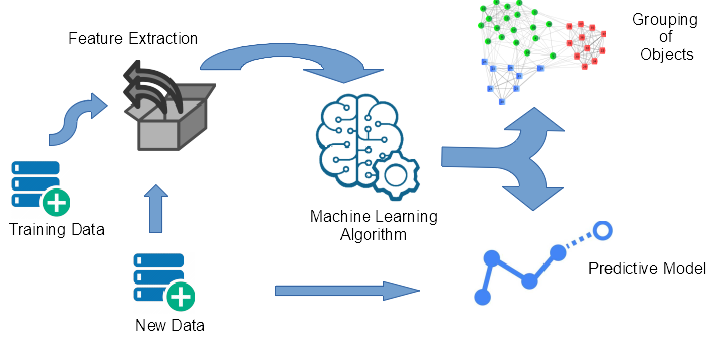
\includegraphics[width=150mm, scale = 1]{images/1_Supervised.png}
	\caption{Supervised Learning Workflow.}
	\label{figure:Supervised_Learning}
\end{figure}

Figure \ref{figure:Supervised_Learning} shows the process of a supervised learning model. The input of the model is data that contains each element with its respective label, next the model extracts the most relevant features of the data, to find the relation between input and output, and construct a logical pattern. Finally, the model after the training step can predict new outputs given a new data without labels.

\subsection{Unsupervised Learning}

Today Big Data is a great tool that makes possible analyze a great amount of information, faster and easier.  Raw data in many cases is difficult to analyze and many cases we do not have an answer key for our trainable data. In this cases we can use unsupervised learning like an alternative, therefore we can determine correlations and identify pattern parsing the available data \cite{Nevala2017}.

This kind of algorithms learns patterns without an explicit feedback (``label'') \cite{Russell2010}, we only have a training data without target values for them \cite{Nilsson1998}. There is no separation of training data and test data \cite{Shai2014}; all the data is the input for the algorithm. Here we have a similitude with the human behavior, when they observe the world, usually they do inferences and group things based on their interaction with the environment, and they are guided by their observations and intuition, this learning is refined exposing to experience and a lot of observations \cite{Nevala2017}.

A the most common technique for this learning is called clustering, \cite{Russell2010} which classify data in meaningful categories, dividing the data into groups with similar characteristics called clusters \cite{Nilsson1998} \cite{Goodfellow2016}. Other techniques are nearest neighbor mapping, singular value decomposition to name a few. Their applications are related to market basket analysis, anomaly/intrusion detection, text classification, identifying like things, sentiment analysis, and so on \cite{Nevala2017} \cite{Halibas2018}.

\begin{figure}[H]	
	\centering
	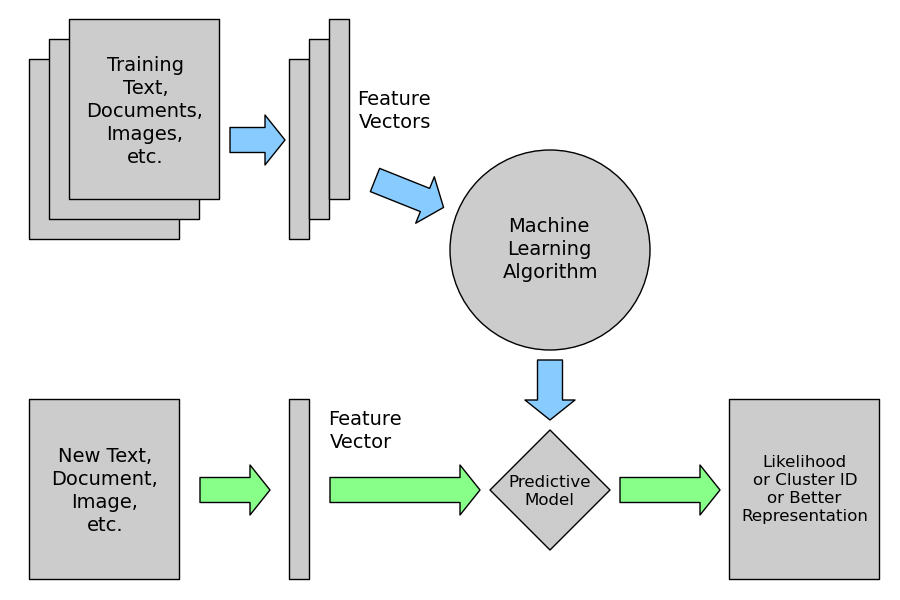
\includegraphics[width=150mm, scale = 1]{images/2-Unsupervised_Learning.png}	
	\caption{Unsupervised Learning Workflow.}	
	\label{figure:Unsupervised_Learning}
\end{figure}

In Figure \ref{figure:Unsupervised_Learning} the features or patterns are extracted of the input data (text, documents, images, etc) data, represented in dimensionality vector, with this data the algorithm is trained. The model created is able use new data to predict outputs like group likelihood or cluster ID.

\section{Neural Networks}
An artificial neural network is a very simplified abstract model of a biological brain, an interconnection of processing units with capability to learn patterns to generalize and associate data. A significant aspect adopted from biological brain is the ``learning capability’’ from the experience and transfer knowledge to find reasonable solutions to similar tasks \cite{ Gurney2004} \cite{ Kriesel2005}.

When we speak about network, it can be referred from a simple single node to a collection of nodes \cite{ Kriesel2005}. The structures of neural networks are basically the next 1) a set of nodes linked associated with a numeric weight that represent the strength of connection between them, 2) an input function for each node that computes the weighted sum of all inputs and 3) an activation function to control the neuron behavior and get the desired output \cite{ Kriesel2005} \cite{Russell2010}. 

\begin{figure}[H]	
	\centering
	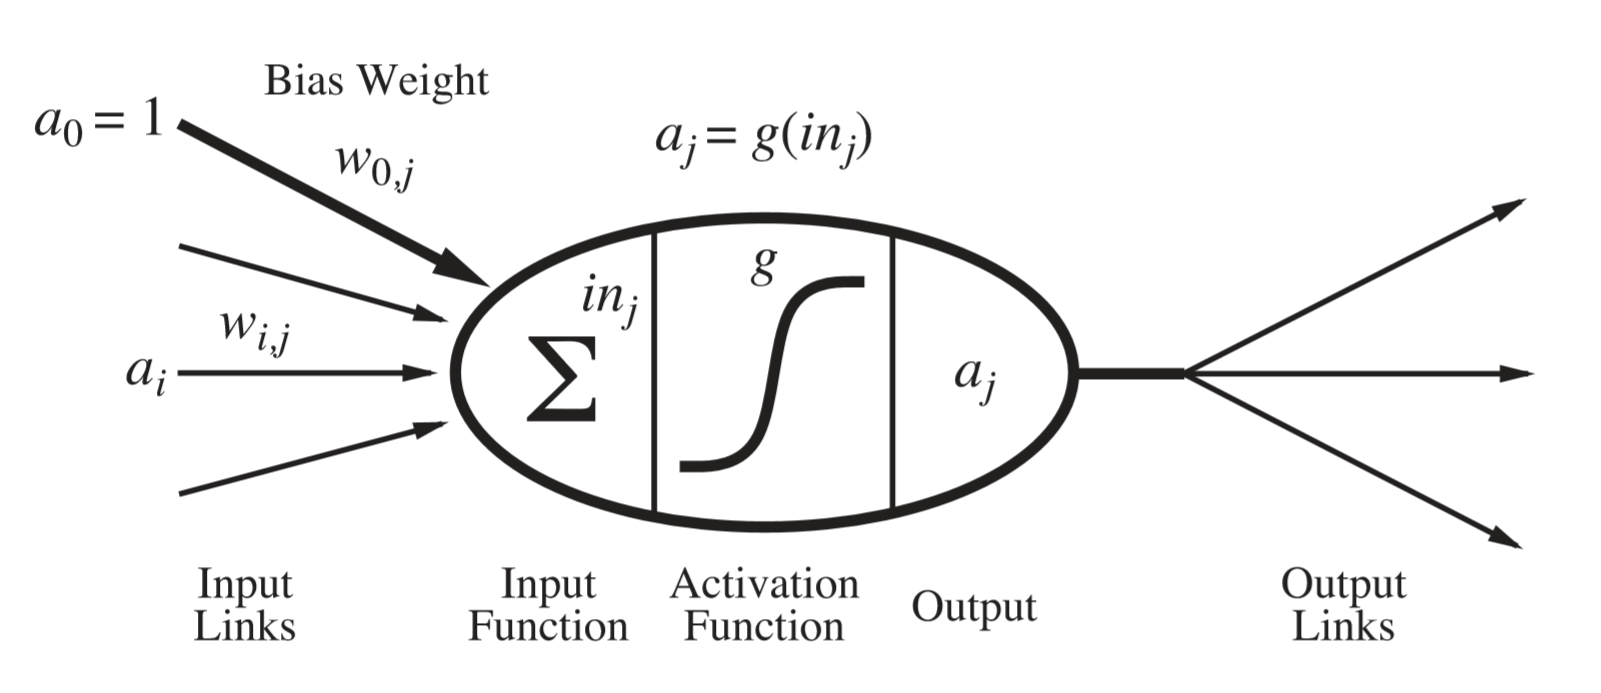
\includegraphics[width=160mm, scale = 1]{images/3_neuron.png}	
	\caption{A Simple Mathematical Neuron Representation \cite{Russell2010}.}	
	\label{figure:Mathematical_Neuron}
\end{figure}

Figure \ref{figure:Mathematical_Neuron} show the basic structure of a simple mathematical neuron, where output is result of apply an activation function (e.g. binary threshold, logistic function, Rectified linear unit function, etc.) to the weighted sum of inputs. The weights are important to minimize the cost of activation function and they are updated when the model is trained. The following equation represent the output after applying an activation function in a neuron showed in Figure \ref{figure:Mathematical_Neuron}.

\begin{equation}
a_j=g\Biggl(\sum_{i=0}^{n} w_{ij}\; a_i\Biggr),
\end{equation}

To form a network, we need connect all these individual neurons like a structure. There are many ways to build the network, feed-forward network and recurrent network are two network topologies very used. The first one showed in Figure \ref{figure:feed-forward-network}, is a network with component clearly separated: an input layer, an output layer and one or more hidden layers also called processing layers. All connections are directed to the following layer and the internal states are just the weights themselves. The second network design the neurons have extra connections adding to a classic feed-forward network, they can be a direct recurrence when the neurons are connected to themselves,  indirect recurrence is a connection to previous layers and a lateral recurrence exist when neurons have connections with another ones at the same layer. These connections influence the neurons itself and their influence depends of the kind of recurrent design. This mean that the network is a dynamic system, the fact that this network feeds its outputs back in its own inputs permit a short-term memory, a model more seem to a brain and by the way, more difficult to understand and build \cite{Kriesel2005} \cite{Russell2010}. 

\def\layersep{5cm}
\begin {figure}[H]
\centering
\resizebox {\textwidth} {!} {
	\begin{tikzpicture}[shorten >=1pt,->,draw=black!100, node distance=\layersep]
	\tikzstyle{every pin edge}=[<-,shorten <=1pt]
	\tikzstyle{neuron}=[circle, fill=red!100, minimum size=20pt,inner sep=0pt]
	\tikzstyle{input neuron}=[neuron, fill=black!100];
	\tikzstyle{output neuron}=[neuron, fill=black!100];
	\tikzstyle{hidden neuron}=[neuron, fill=black!100];
	\tikzstyle{hidden1 neuron}=[neuron, fill=black!100];
	\tikzstyle{annot} = [text width=4em, text centered]
	
	% Draw the input layer nodes
	\foreach \name / \y in {1,...,3}
	% This is the same as writing \foreach \name / \y in {1/1,2/2,3/3,4/4}
	\node[input neuron] (I-\name) at (0,-6+\y) {};
	
	% Draw the hidden layer nodes
	\foreach \name / \y in {1,...,8}
	\path[yshift=0.5cm]
	node[hidden1 neuron] (H-\name) at (\layersep,-\y cm) {};
	
	% Draw the hidden layer nodes
	\foreach \name / \y in {1,...,8}
	\path[yshift=0.5cm]
	node[hidden neuron] (H-\name) at (\layersep,-\y cm) {};
	
	% Draw the output layer node
	\node[output neuron,pin={[pin edge={->}]right:Output}, right of=H-3] (O) {};
	
	% Connect every node in the input layer with every node in the
	% hidden layer.
	\foreach \source in {1,...,3}
	\foreach \dest in {1,...,8}
	\path (I-\source) edge (H-\dest);
	
	% Connect every node in the hidden layer with the output layer
	\foreach \source in {1,...,8}
	\path (H-\source) edge (O);
	
	% Annotate the layers
	\node[annot,above of=H-1, node distance=1cm] (hl) {Hidden layer};
	\node[annot,left of=hl] {Input layer};
	\node[annot,right of=hl] {Output layer};
	\end{tikzpicture}
}
\caption{Feed Forward Network}
\label{figure:feed-forward-network}
\end{figure}


\section{Deep Learning}

The artificial intelligence usually solves problems intellectually challenge for the humans relatively easy, but the task the human performs easy or solve intuitively are very difficult for the computers. The problems like speech recognition or applications to find faces in images are challenge task. For these problems we must allow computers gather knowledge from the experience, avoiding specify all the knowledge that the system needs. It means build a complicated task using more simpler concepts \cite{Goodfellow2016}.

\ac{DL} has great advancement in many fields of \ac{AI}, like Natural Language Processing, Speech Recognition, Computer Vision, Biomedical Applications and so on \cite{Chandra2017}

These concepts form a deep graph, including many layers, the reason for that this approach is known how Deep Learning \cite{Goodfellow2016}.

\ac{MLP} or feedforward deep layer is the most typical example of deep learning approach. \ac{MLP} consists in an input layer, that contains the input data for the model, next we have the hidden layers, a variable number of neurons and layers, and finally an output layer as is showed in the Figure \ref{figure:MLP}. That depth (hidden layers) allows to learn a multi-step program.

\begin{figure}[H]	
	\centering
	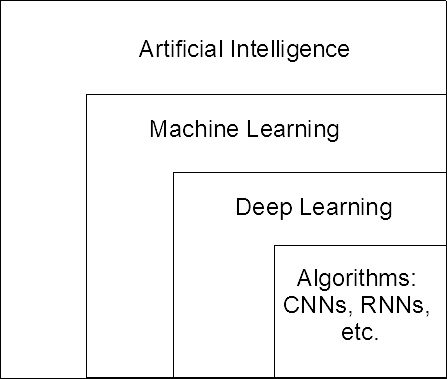
\includegraphics[width=85mm]{images/2-AI.png}
	\caption{Artificial Intelligence Landscape}
	\label{figure:AI}
\end{figure}

Figure \ref{figure:AI} shows the \ac{AI} landscape, when \ac{DL} is a kind of \ac{ML}, which is used for many approaches of \ac{AI}.

There are many algorithms of Deep Learning, like \ac{CNN} used commonly when is working with images and \ac{RNN} to process sequences of data essentially.

\subsection{Convolutional Neural Networks}

\ac{CNN} is applied to problems with a grid-like topology, a clear example of this type of data are the images, other are the regular time intervals. \ac{CNN} formally is composed with a mathematical operation called convolution in at least one layer, instead of a general matrix operation \cite{Goodfellow2016}. \ac{CNN} is very used in recognition, as a powerful visual model, to extract features in a hierarchy of concepts. \cite{Long2015}.

Historically this type of network was some the firsts in solve important commercial problems \cite{Goodfellow2016} like the handwritten zip code recognition.

\subsection{Recurrent Neural Networks}

\ac{RNN} is a kind of networks to processing sequential data. They are very powerful because they store efficiently information about the past. They are specialized in process a sequence of values  \cite{Goodfellow2016}, mapping all the previous input to each output. This allows the memory of old inputs can persist and influence in the next network output \cite{Graves2017}.

\ac{RNN} are used for resolving many types of problems, \cite{Chandra2017} proposes a method to improving the use of \ac{RNN} in classification of images. In other hand, \ac{RNN} is also used to detection and diagnosis of a chemical process that show results with excellent performance \cite{Xavier2018}.

\section{Natural Language Processing}
\section{Text Similarity}
\subsection{Lexical Similarity}
\subsection{Semantic Similarity}

\chapter{Methodology} \label{chapter 3}
\section{Description}
\section{Formalization}
\section{Data Processing Pipeline}

\chapter{Similarity Analysis} \label{chapter 4}
\section{Deep Learning Framework}
\section{Model Description}
\section{Model Architecture}

\chapter{Experiments} \label{chapter 5}
\section{Hardware} 
\section{Software}
\section{Experimental Results}

\chapter{Conclusion and Future Work} \label{chapter 6}
In summary, more text here

%\chapter*{References} 
%\addcontentsline{toc}{chapter}{Bibliography}
\bibliographystyle{unsrt}
\bibliography{references} 
%\printbibliography[heading=none, ]

\begin{appendices}
\chapter{GitHub Repositories}
The GitHub repositories of the big data and machine learning deamon are avaliable upon request at danny.villanueva1@upr.edu. The following sections contain the links.

\section{Big Data Platform}
https://github.com/THSUPRM/bigdata/tree/master/python

\subsection{Machine Learning Platform}
https://github.com/THSUPRM/bigdata/tree/master/DetectDiseaseTHS/ths
\end{appendices}

\end{document}